\documentclass[a4paper,11pt]{article}
%@@@@@@@@@@@@@@@@@@@@@@@@@@@@@@@@@@@@@@@@@@@@@@@@@@@@@@@@@@@
%@@@@@@@@@@@@@@@@      PACOTES BÁSICOS		     @@@@@@@@@@
%@@@@@@@@@@@@@@@@@@@@@@@@@@@@@@@@@@@@@@@@@@@@@@@@@@@@@@@@@@@

\usepackage[T1]{fontenc}
\usepackage[utf8]{inputenc}
\usepackage{lmodern} 
\usepackage[portuguese]{babel}
\usepackage{amsmath}
\usepackage{array}
\usepackage{graphicx}				%para imagens
\usepackage{epstopdf} 				%resolve problemas eps-pdf
\usepackage{pict2e}				%%writting to images
%@@@@@@@@@@@@@@@@@@@@@@@@@@@@@@@@@@@@@@@@@@@@@@@@@@@@@@@@@@@
%@@@@@@@@@@@@@@@@     PACOTES NÃO TAOBÁSICOS		 @@@@@@@@@@
%@@@@@@@@@@@@@@@@@@@@@@@@@@@@@@@@@@@@@@@@@@@@@@@@@@@@@@@@@@@
\usepackage{fancyhdr}				% para o cabeçalho bonito
\usepackage{caption}					%para legendas
\usepackage{subcaption}				% e sublegendas
\usepackage{placeins} 				%controlar o lugar dos floats
\pagestyle{fancy} 					% número de pag e cabeçalho
\usepackage{txfonts} 				%fontes bonitas? acho que para o título
\usepackage[usenames]{color} 		% algo com gunplot e eps
\usepackage{ifthen}
\usepackage{xparse}
\graphicspath{{./../images/}{./../data/}{./graph/}}	% procura imagens nessa pasta
\usepackage{float} %%para definir ambiente gráfico
\newfloat{Gráfico}{hbtp}{lop}[section]
%\usepackage{undertilde}	%%para notação de vetor do yuri
\usepackage[import]{xy} % para escrever em imagens
\xyoption{import}

\usepackage{listings}
\lstset{frame=single,}
%@@@@@@@@@@@@@@@@@@@@@@@@@@@@@@@@@@@@@@@@@@@@@@@@@@@@@@@@@@@
%@@@@@@@@@@@@@@@@      Cabeçalho de cada página      @@@@@@@
%@@@@@@@@@@@@@@@@@@@@@@@@@@@@@@@@@@@@@@@@@@@@@@@@@@@@@@@@@@@
\setlength{\headheight}{25pt}%compila sem erro
	\fancyhead{}
	\fancyfoot{}
	\fancyhead[R]{Sistemas de Medição}%direito superior
	\fancyhead[L]{
\includegraphics[height=0.25in]{./../images/logo_unb.pdf}}%esquerda superior
	\fancyfoot[C]{\thepage}%baixo centro
%E: Even page, O: Odd page, L: Left field, C: Center field, R: Right field, H: Header, F: Footer
% em documentos com dois lados use LO, RO. como esse documento não tem lados essa opção é inútil


%@@@@@@@@@@@@@@@@@@@@@@@@@@@@@@@@@@@@@@@@@@@@@@@@@@@@@@@@@@@
%@@@@@@@@@@@@@@@@      NOVOS COMANDOS		      @@@@@@@@@
%@@@@@@@@@@@@@@@@@@@@@@@@@@@@@@@@@@@@@@@@@@@@@@@@@@@@@@@@@@@
\newcommand\undermat[2]
	{
	  \makebox[0pt][l]
	  	{$\smash{\underbrace{\phantom{%
    \begin{matrix}#2\end{matrix}}}_{\text{$#1$}}}$
    		}#2
    	}
    	
\newcommand{\HRule}
	{
	\rule{\linewidth}{0.5mm}
	}
	
\newcommand{\EmptyPage}
	{
	\thispagestyle{empty}
	\mbox{ }
	\newpage	
	} 
	
\newcommand{\MakeMyTitlePage}[4]
%%Argumentos: 
%1º Nome da Matéria
%2º subtítulo ex: experimento IV
%3º título
%4º autores
% exemplo de autores:
%	\begin{center} \large
%		\begin{tabular}{llr} \
%		& & \\[0.05cm]		
%		Professora & Nadia Maria de Liz Koche & \\
%		
%		Alunos:& & \\
%		& Juarez A.S.F 					& 11/0032829\\
%		& Sérgio Fernandes da Silva Reis & 11/0140257\\
%		& Jedhai Pimentel				& 09/0007883\\	[0.05cm]	
%		\end{tabular}
%	\end{center}
{
\begin{titlepage}
\begin{center}

% Upper part of the page. The '~' is needed because \\
% only works if a paragraph has started.

\includegraphics[width=\textwidth]{./../images/logo_unb.pdf}~\\[1cm]

\Huge #1\\[0.5cm]

\huge #2

% Title
\HRule \\[0.4cm]
{ \huge \bfseries  #3}\\[0.4cm]

\HRule \\[0.5cm]

{\large \today}


\vfill %%o que vier depois vai ao fim da páginda


%Autor e Professor
\begin{center} \large
#4
\end{center}

\end{center}
\end{titlepage}

\EmptyPage
\tableofcontents
\newpage

}
	
%@@@@@@@@@@@@@@@@@@@@@@@@@@@@@@@@@@@@@@@@@@@@@@@@@@@@@@@@@@@
%@@@@@@@@@@@@@@@@      NOVOS AMBIENTES		      @@@@@@@@@
%@@@@@@@@@@@@@@@@@@@@@@@@@@@@@@@@@@@@@@@@@@@@@@@@@@@@@@@@@@@
\newcounter{graph-c}
\setcounter{graph-c}{0}


%\NewDocumentEnvironment{Graph}{m}
 % {%antes
  %\addtocounter{graph-c}{1}
  %\begin{figure}
  %}
 %{
 %depois
%	\end{figure} 
%	\caption*{Grafico \arabic{graph-c} - #1}
 %}

















%inclui todosos pacotes utilizados

\newcommand{\MyBox}[1]
{
	\begin{tabular}{|l|}\hline
	  #1 \\ \hline	    
	\end{tabular} 	
}

\begin{document}



\MakeMyTitlePage
{Física Experimental 4}
{Experimento V}
{Espectroscopia Ótica}
{%autores
		\begin{tabular}{llr} \
		& & \\[0.05cm]		
		Professora & Nadia Maria de Liz Koche & \\
		
		Alunos:& & \\
		& Juarez A.S.F 					& 11/0032829\\
		& Sérgio Fernandes da Silva Reis & 11/0140257\\
		& Jedhai Pimentel				& 09/0007883\\
	[0.05cm]	
		\end{tabular}
}

%@@@@@@@@@@@@@@@@@@@@@@@@@@@@@@@@@@@@@@@@@@@@@@@@@@@@@@@@@@@
%@@@@@@@@@@@@@@@@      OBJETIVOS      @@@@@@@@@@@@@@@@@@@@@@
%@@@@@@@@@@@@@@@@@@@@@@@@@@@@@@@@@@@@@@@@@@@@@@@@@@@@@@@@@@@
\section{Objetivos}
 \paragraph{}Estudar difração de luz monocromática em fendas simples, duplas
 múltipla e rede de difração. Determinar os comprimentos de ondas presentes
 no espetro de lâmpada de Mercúrio.
%@@@@@@@@@@@@@@@@@@@@@@@@@@@@@@@@@@@@@@@@@@@@@@@@@@@@@@@@@@@
%@@@@@@@@@@@@@@@        MATERIAIS         @@@@@@@@@@@@@@@@@@
%@@@@@@@@@@@@@@@@@@@@@@@@@@@@@@@@@@@@@@@@@@@@@@@@@@@@@@@@@@@
\section{Materiais}
\paragraph{} Para o experimento utiliza-se:
\begin{itemize}
	\item[•]Fonte de Laser He-Ne
	\item[•]Lâmpada de vapor de Hg
	\item[•]Diafragma
	\item[•]Slide de fenda dupla de largura 0.1mm e espaçamentos 0.175mm
	\item[•]Slide de fenda dupla de largura 0.1mm e espaçamentos 0.150mm
	\item[•]Slide de fenda dupla de largura 0.1mm e espaçamentos 0.300mm
	\item[•]Slide de múltiplas fendas de densidade 80 fendas/cm
  \item[•]Slide de múltiplas fendas de densidade 100 fendas/cm
  \item[•]Slide de múltiplas fendas de densidade 300 fendas/cm	
	\item[•]Rede de difração 600 fendas/mm
	\item[•]Suporte para slides
	\item[•]Anteparo fixo com papel milimetrado
	\item[•]Banco ótico,
	\item[•]Espectroscópio,
	\item[•]Régua milimetrada.
\end{itemize}  
%@@@@@@@@@@@@@@@@@@@@@@@@@@@@@@@@@@@@@@@@@@@@@@@@@@@@@@@@@@@
%@@@@@@@@@@@@@@        INTRODUCAO       @@@@@@@@@@@@@@@@@@@@ %@@@@@@@@@@@@@@@@@@@@@@@@@@@@@@@@@@@@@@@@@@@@@@@@@@@@@@@@@@@
\newpage
\section{Introdução}
\paragraph{}Difração é o efeito que ocorre quando a luz ao passar por
um obstáculo tem a sua trajetória desviada. Pontos que não seriam
iluminados caso a luz passasse em linha reta pelo obstáculo passam
a ser devido a esse efeito. O fenômeno pode ser explicado pelo princípio
de Huygens que diz que cada ponto de uma frente de onda funciona como uma
fonte pontual de mini-ondas. A figura \ref{fig:intro-huygens} ilustra como 
o princípio é usado para achar a nova frente de onda. 

\paragraph{}Além do espalhamento outro efeito interessante ocorre. 
Ao colocarmos uma tela após a fenda não só observamos que a área
iluminada é maior que a fenda mas também o padrão como a intensidade
de luz se distribui não é constante nem é um máximo central que decai 
com a distância ao centro como poderia se esperar.
 A figura \ref{fig:single-slit-pattern}
ilustra o padrão observado, nela vemos a tela em branco e os picos
de luz em escuro. Notamos um máximo central ladeado de máximos
secundários separados por regiões de intensidade nula. A distribuição 
lembra o padrão de gerado por interferência de duas fendas e não
é coincidência, a origem dos efeitos é a mesma: a interferência.
Voltando ao princípio de Huygens cada ponto da fenda funciona como
uma fonte pontual e a luz de cada um desses pontos deve interferir
com a luz dos outros pontos da fenda na tela. Onde essa interferência for
construtiva vemos os máximos, quando destrutiva vemos os 
mínimos.

\paragraph{} Análise detalhada de como essa interferência ocorre
num caso mais geral é complicada mas se a tela de captura for tomada
muito distante algumas simplificações são válidas e observamos o padrão
de difração de Fraunhofer. Considerando as grandezas indicadas na figura
\ref{fig:single-slit-schematic} pode-se mostrar que a posição
 angular dos mínimos $\theta _{dark}$ 
é tal que:
\begin{equation}
	\begin{array}{ll}
	a \sin \theta_{dark} = \mbox{m}\lambda & \mbox{, m =}
				 \pm 1, \pm 2, \pm 3, \ldots	
	\end{array}
	\label{eq:single-slit}
\end{equation}
 
\paragraph{}Pode-se ainda mostrar que para a difração em fenda única nos
 critérios de Fraunhofer a distribuição de intensidade segue a fórmula:
\begin{equation}
	I(\theta) =
	 I_{max} \left[
	 			\frac{
	 				sin\left(
	 					\frac{\pi a sin \theta}{\lambda}
	 					\right)
	 				}
					{
					\frac{\pi a sin \theta}{\lambda}
					}
				\right]^2
	\label{eq:single-slit-intensity-pattern}
\end{equation}
\paragraph{} O estudo da difração em fenda dupla deve levar com
 conta a interferência da luz difratada em uma fenda com a
 outra e a interferência entre os pontos da
própria fenda segundo o princípio de Huygens.
 A figura \ref{fig:double-slit-schematic}
mostra as grandezas importantes para o processo.
A interferência entre as duas fendas separadas por d
 nos dá a posição dos máximos em:
\begin{equation}
	\begin{array}{ll}
		d sin \theta _{max} = m \lambda & \mbox{, m =} 0,
					 \pm 1, \pm 2, \ldots  
	\end{array}
	\label{eq:maximos-fenda-dupla-sem-difracao}
\end{equation}

\paragraph{}Vale a pena notar que esse é o resultado dos máximos previstos
levando em consideração apenas a interferência de uma fenda com a outra. 
O estudo do padrão de intensidade em fendas duplas levando em consideração
também a interferência entre os pontos de uma mesma fenda nos dá:
\begin{equation}
	I(\theta) =
	 I_{max} 
	    \underbrace
	      {
	      \left[
	 			\frac{
	 				sin\left(
	 					\frac{\pi a sin \theta}{\lambda}
	 					\right)
	 				}
					{
					\frac{\pi a sin \theta}{\lambda}
					}
				\right]^2
				}_\textrm{fator de difração}
				\cdot
				\underbrace
				{
				cos^2 
				  \left(
				      \frac
				        {\pi d sin \theta}
				        {\lambda}
				  \right)
				}_\textrm{fator de interferência entre as fendas}
	\label{eq:doble-slit-intensity-pattern}
\end{equation}

\paragraph{}Note que o efeito final é uma composição do efeito de interferência
de duas fendas com a difração em fenda única,
 sendo a segunda um envelope para a primeira.
A figura \ref{fig:double-slit-patter} ilustra
 a curva de interferência. Veja que existem máximos
previsto pela fórmula \ref{eq:maximos-fenda-dupla-sem-difracao}
 que são achatados pelo envelope da 
difração e aparecem como mínimos.

\paragraph{} Temos ainda a interferência em redes de difração.
 Quando tivermos múltiplas fendas cada
uma irá interferir em todas as outras produzindo um padrão de difração
que é caracterizado pela densidade
de fendas N. O padrão observado é mostrado na figura
\ref{fig:mult-slit-pattern}.Como pode ser
visto na figura temos estreitos e poucos máximos principais e
numerosos máximos secundários. Os
máximos principais podem ser achados pela fórmula:
\begin{equation}
    \begin{array}{ll}
    d sin \theta = m \lambda & \mbox{, m = } 0, \pm 1, \pm 2, \ldots
   \end{array}
\label{eq:rede}
\end{equation}

\paragraph{}Onde d é a distância entre duas fendas adjacente e pode
ser determinado por $d = \frac{1}{N}$.  Vemos que os ângulos
nos quais os máximos são observados dependem do 
comprimento de onda $\lambda$ da luz incidente.
Caso um feixe incidente contenha 
vários comprimentos de onda, estes serão divididas
ao passarem por uma rede de difração.
Esse comportamento é utilizado para determinar
o material atômico que produziu um dado feixe
de luz. Sabe-se que as frequência emitidas por um
átomo estão relacionadas com os saltos quânticos
sofrido pelos seus elétrons. Pelo modelo atômico de Bohr
esses saltos estão restritos a determinados valores
de energia e são característicos de cada átomo. Uma
análise do espectro da luz emitida por um dado
material pode então nos dizer que material é este.
É assim que podemos saber, por exemplo, o material
constitutivo das estrelas ou ainda de um gás a baixa
pressão preso em um recipiente sobre o qual se aplica 
tensão elétrica.
\FloatBarrier
\begin{figure}[H]

	\begin{subfigure}[!htp]{0.5\textwidth}
		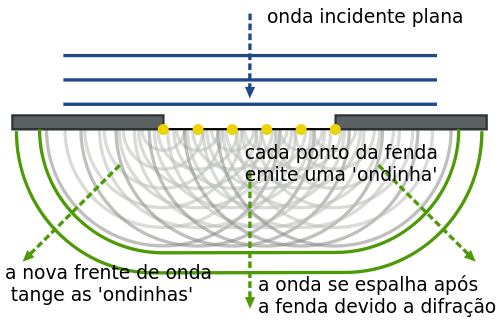
\includegraphics[width = 6 cm]{./images/Huygens-Principle.png}
		\caption{Princípio de Huygens para explicar a difração}
		\label{fig:intro-huygens}
	\end{subfigure}
\hspace{1 cm}	
	\begin{subfigure}[!htp]{0.5\textwidth}
		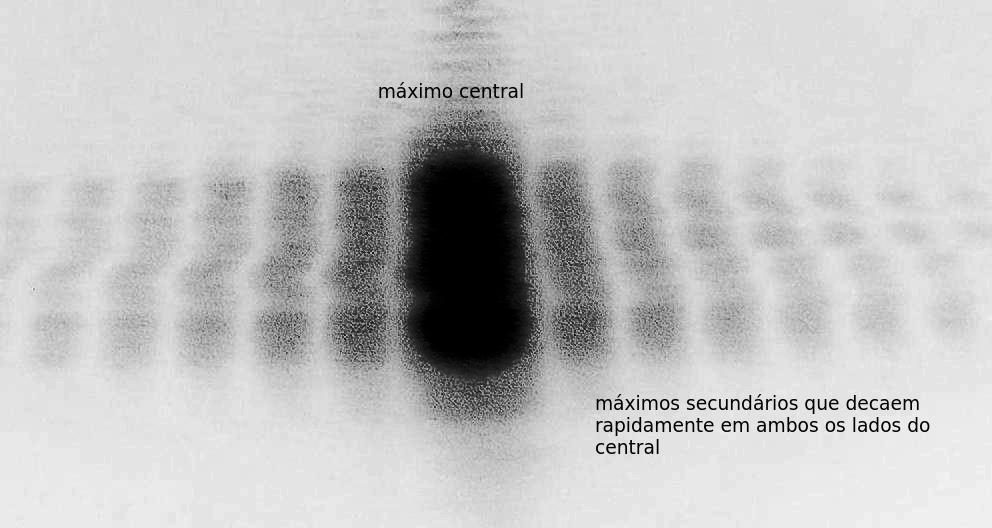
\includegraphics[width = 8 cm]{./images/single-slit-pattern.jpg}
		\caption{Padrão experimental de difração em fenda simples}
		\label{fig:single-slit-pattern}
	\end{subfigure}
%
\vspace{1 cm}
%
	\begin{subfigure}[!htp]{0.5\textwidth}
	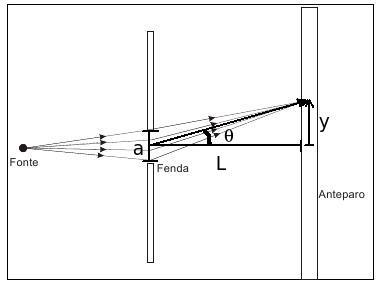
\includegraphics[width = 6 cm]{./images/single-slit-schematic.jpg}
		\caption{grandezas importantes para a difração em fenda simples}
		\label{fig:single-slit-schematic}
	\end{subfigure}
\hspace{1 cm}	
	\begin{subfigure}[!htp]{0.5\textwidth}
	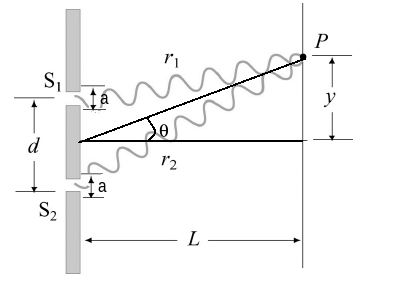
\includegraphics[width = 6 cm]{./images/MIT-double-slit-schematic.png}
		\caption{grandezas importantes para a difração em fenda dupla}
		\label{fig:double-slit-schematic}
	\end{subfigure}
%
\vspace{1 cm}
%
\hspace{-1 cm}	
	\begin{subfigure}[!htp]{0.5\textwidth}
		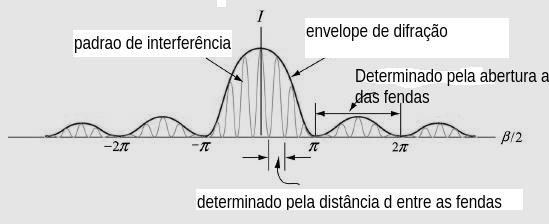
\includegraphics[width = 8 cm]{./images/MIT-figure.jpg}
		\caption{Padrão de intensidade em fenda dupla}
		\label{fig:double-slit-patter}
	\end{subfigure}
\hspace{2 cm}	
	\begin{subfigure}[!htp]{0.5\textwidth}
		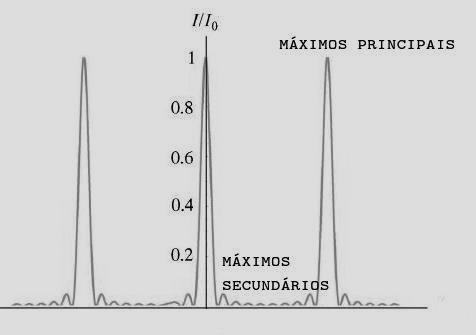
\includegraphics[width = 6 cm]{./images/MIT-mult-slit.jpg}
		\caption{Padrão de intensidade em múltiplas fendas (N = 10)}
		\label{fig:mult-slit-pattern}
	\end{subfigure}

	\caption{Difração em diferentes tipos de fenda}

\end{figure}

\FloatBarrier
%@@@@@@@@@@@@@@@@@@@@@@@@@@@@@@@@@@@@@@@@@@@@@@@@@@@@@@@@@@@
%@@@@@@@@@@@@       PROCEDIMENTOS        @@@@@@@@@@@@@@@@@@@
%@@@@@@@@@@@@@@@@@@@@@@@@@@@@@@@@@@@@@@@@@@@@@@@@@@@@@@@@@@@
\section{Procedimentos}

\paragraph{Fenda Simples}Monta-se o banco ótico como na
figura \ref{fig:montagem}
primeiramente utilizando o diafragma na montagem. 
Liga-se o laser de He-Ne e ajusta-se a posição do suporte e da tela para
que se obtenha um padrão nítido de difração. Anota-se a distância D entre 
a fenda e a tela. Um papel milimetrado é preso à tela de captura para que
os padrões possam ser anotados. Variando-se a abertura do diafragma os padrões
obtidos são desenhados no papel milimetrado tomando-se atenção para representar
a posição, largura e intensidade das franjas luminosas. 

\paragraph{Fenda dupla} A montagem é feita agora usando slides de fenda dupla.
Ajusta-se o sistema para que o laser incida sobre as duas fendas e para que
a imagem obtida na tela seja nítida. O padrão obtido na tela é então anotado no
papel milimetrado. Procedimento é repetido para
três diferentes slides cada um com
uma distância entre fendas diferente.
Anotam-se os valores nominais de abertura de fenda
e distância entre fendas de cada slide.

\paragraph{Fenda múltiplas} A montagem é
feita utilizando-se agora slides com diferentes
densidade de fendas. As densidades utilizadas são da ordem de 
dezenas de fendas por cm.
Os padrões obtidos são desenhados no papel milimetrado novamente 
prestando-se atenção para a posição, largura e intensidade dos máximos.

\paragraph{Redes de Difração} O procedimento é feito novamente mas utilizando-se
densidade de fendas da ordem de centenas de fendas por
mm. Mede-se as 'alturas' dos máximos
para que se possa determinar os ângulos de máximo e
posteriormente a densidade de ranhuras
experimentalmente.

\paragraph{Determinação de espectros} Passamos agora para a montagem do 
espectroscópio na figura \ref{fig:montagem2}. A lâmpada utilizada é 
de mercúrio a baixa pressão e a rede de difração possui densidade nominal de
600 linhas/mm. O foco do telescópio
e a abertura da fenda são ajustados para que se tenha 
uma imagem nítida da fenda. Fazendo o telescópio alinhado com a fonte mede-se
o ângulo marcado na mesa, esse será o zero nas nossas medidas.
Varia-se então a posição angular do telescópio e anotam-se 
as posições onde a fenda volta a aparecer e a sua respetiva cor
nessa condição. Os ângulos medidos são anotados com os valores
em que aparecem na mesa, após a coleta de dados subtrai-se o
valor do ângulo para a posição 0 definida inicialmente para
obter a variação angular a ser utilizada nos cálculos.


\paragraph{Dispersão em um prisma}
O procedimento anterior é refeito mas colocando
um prisma no lugar da rede de difração. O prisma é colocado
de forma que sua base triangular fique apoiada sobre a mesa
e que o feixe colimado incida sobre sua ponta. Isso é feito
para que a dispersão da luz ocorra horizontalmente e não
verticalmente. Com o telescópio procura-se as posições
angulares em que o feixe é visível e a sua cor.

\FloatBarrier

\begin{figure}
  \begin{subfigure}{0.5\textwidth}
	    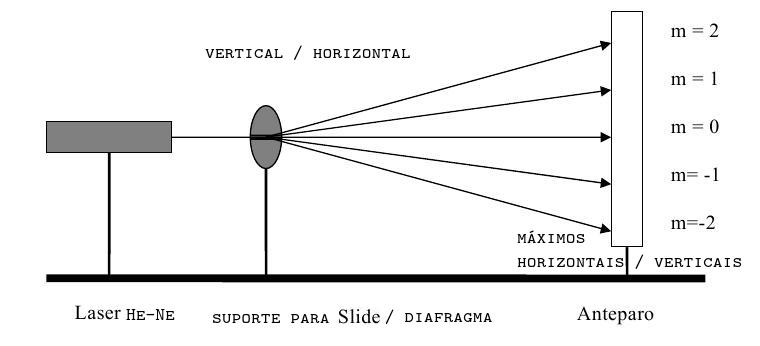
\includegraphics[width = 12 cm]{./images/montagem1.jpg}
	    \caption{procedimentos em banco ótico}
	    \label{fig:montagem}
	\end{subfigure}
	
	  \begin{subfigure}{0.5\textwidth}
	    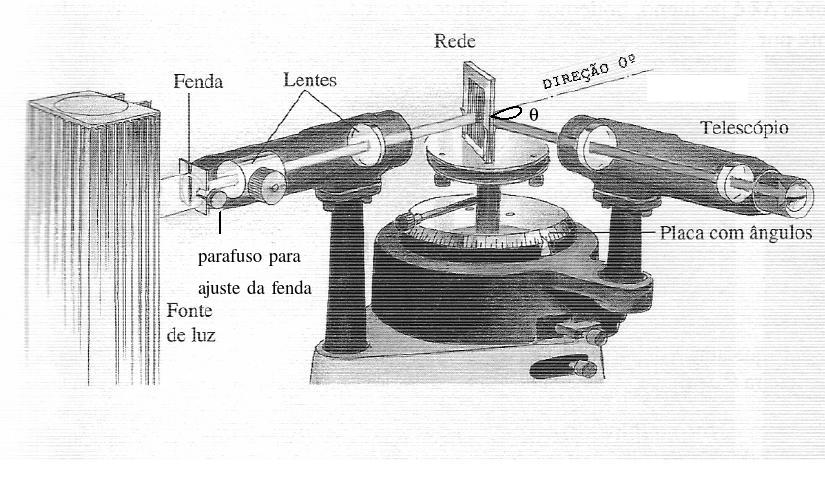
\includegraphics[width = 12 cm]{./images/montagem2.jpg}
	    \caption{procedimento em espetroscópio de rede}
	    \label{fig:montagem2}
	\end{subfigure}
	
	\caption{montagem dos procedimentos}
\end{figure}
 \FloatBarrier
%@@@@@@@@@@@@@@@@@@@@@@@@@@@@@@@@@@@@@@@@@@@@@@@@@@@@@@@@@@@
%@@@@@@@@@@@@@@@@@@@       DADOS      @@@@@@@@@@@@@@@@@@@@@@
%@@@@@@@@@@@@@@@@@@@@@@@@@@@@@@@@@@@@@@@@@@@@@@@@@@@@@@@@@@@
 \newpage
\section{Dados}
\paragraph{}Os papéis milimetrados em anexo ao relatório nos
mostram os padrões obtidos experimentalmente.
Os dados dessa seção foram obtidos a partir de medidas retiradas
destes papeis.
\subsection{Caracterização da difração em fenda única}


\paragraph{}Observamos que a intensidade da fenda principal diminui na
proporção em que a sua largura aumenta, e as intensidades
caem também com o número, m, da franja. Estas coisas
acontecem de forma proporcional a redução do tamanho da
fenda, assim, quanto menor a fenda for, maior a largura da
franja e menor a intensidade.   

\paragraph{}
Para os três padrões anotados a tabela a seguir mostra a largura $L_n$
dos máximos centrais:

\begin{table}[!htp]
    \centering
    \begin{tabular}{|l|}\hline
      $L_1$ = 2.30 cm $\pm 0.05$ cm\\ \hline
      $L_2$ = 1.50 cm $\pm 0.05$ cm\\ \hline
      $L_3$ = 3.70 cm $\pm 0.05$ cm\\ \hline
    \end{tabular}
\caption{Largura dos máximos centrais}
\end{table}


\paragraph{}Aqui a distância D medida da fenda ao anteparo é:
\begin{table}[!htp]
    \centering
    \begin{tabular}{|l|}\hline
      D = 213.0 cm $\pm 0.2$ cm\\ \hline
    \end{tabular}
\end{table}


\subsection{Caracterização da difração em fenda dupla}
\paragraph{}
Diferente da fenda simples, os pontos observados são menos
achatados. Notamos que a distancia entre os máximos aumentam
e a sua largura diminui a medida que as distancia entre as
duas fendas diminui. A largura, diferente do primeiro caso
onde aumentava a medida que as franjas se distanciavam, aqui
elas diminuem a medida que as franjas se afastam. 

\paragraph{}Neste procedimento usou-se slides de fendas duplas todas
com abertura a de:

\begin{displaymath}
	a = 0.1 mm
\end{displaymath}

\paragraph{}A tabela a seguir mostra a distância y
ao máximo central para alguns m's para os 4 pares de fendas
utilizados com suas respectivas distância entre fendas D:

 \begin{table}[!htp]
    \centering
    \begin{tabular}{|l|l|l|l|l|}\hline
	Dupla	& $y_{max 1} \pm 0.5mm$ &  $y_{max 2}
\pm 0.5mm$ & $y_{max 3} \pm 0.5mm$ & $y_{max 4} \pm 0.5mm$ \\ \hline
      	1ª (D = 0.150mm) &5.5mm &13.0mm &26.0mm & 33.5mm \\ \hline
      	2ª (D = 0.175mm) &5.5mm &12.5mm & 18.5mm &25.5mm \\ \hline
      	3ª (D = 0.200mm) &5.5mm &15.0mm & 25.0mm & - \\ \hline
	4ª (D = 0.300mm) &3.5mm &6.5mm &13.5mm & 16.5mm \\ \hline
	5ª (D = 2.000mm) &10.0mm &- &- &- \\ \hline
\end{tabular}
\caption{alguns máximos para os pares de fendas estudados}
\label{tab:fendas-multiplas}
\end{table}


\paragraph{}Para as 4 primeiras duplas de fendas a distância
do slide até o anteparo foi de $L = 2.000m \pm 0.025m$. 
Para o último caso precisou-se aproximar a tela da fenda
para que os pontos pudesse ser marcados. Nesse caso mediu-se
$L = (84.0 \pm 0.1)cm $. Os erros nas medidas dos L's se deve a dois motivos:
no primeiro caso precisou-se usar 3 réguas milimetradas para se 
medir a distância e a medida foi feita de forma indireta
subtraindo-se duas posições; no segundo caso usou-se apenas uma, mas
novamente a medida foi feita indiretamente pela subtração da medida
de duas posições, a do anteparo e a do suporte para 
slide. 



\subsection{Caracterização de fendas múltiplas}

\paragraph{}Aqui, quase não se nota a diferença de
intensidade nos máximos medidos e nas  larguras de fendas e
elas são mais igualmente espaçadas.



\paragraph{} Medimos no papel milimetrado a distância do
primeiro máximo ao máximo central. Os valores obtidos foram:
\begin{table}[!htp]
    \centering
    	\begin{tabular}{|l|l|}\hline
   		densidade de fendas (fendas/cm) & $(y_{1} \pm 0.5)mm$ \\ \hline
		80	& 10.5 mm  \\ \hline
		100	& 13.5  mm\\ \hline

	\end{tabular}
  \caption{primeiros máximos para fendas múltiplas}
\label{tab:multiplas}
\end{table}


\subsection{Caracterização de redes de difração}

\paragraph{}Os máximos observados no procedimento com rede de difração
de densidade de ranhuras nominal 600 linhas/mm são listados na tabela a seguir:
\begin{table}[!htp]
    \centering
    	\begin{tabular}{|l|l|}\hline
   		ordem n & $y_{máx n} \pm 0.5mm$ \\ \hline
		0	& 0.0 mm  \\ \hline
		1	& 35.0mm\\ \hline
		2	& 99.5mm\\ \hline
	\end{tabular}
  \caption{máximos para rede de difração 600 l/mm}
\label{tab:rede}
\end{table}

\paragraph{} A distância do slide a tela L é:

\begin{displaymath}
	L = (9.00 \pm 0.05) cm
\end{displaymath}


\subsection{Determinação de espectros}
\paragraph{} O ângulo marcado na mesa quando o telescópio está alinhado
com a fonte é:
\begin{center}
  \begin{tabular}{|l|}\hline
      $\theta _0 = (55.50 \pm 0.05)º$
      \\ \hline
  \end{tabular}
\end{center}

\paragraph{} Os ângulos marcados pela mesa $\theta_{medido}$
e a variação do ângulo$\triangle \theta$ em relação ao inicial
quando a fenda volta a aparecer e as respectivas cores observadas são:
\begin{table}[!htp]
    \centering
    \begin{tabular}{|l|l|l|}\hline
        $ \theta_{medido}\pm 0.05º$ &$\triangle \theta \pm 0.1º$ & cor \\ \hline
        69.50º & 14.0º  &roxo\\ \hline
        70.60º & 15.1º  &azul\\ \hline
        72.60º & 17.1º  &verde \\ \hline
        74.60º & 19.1º  &verde escuro\\ \hline
        75.70º & 20.1º  &laranja\\ \hline
        
        84.70º & 29.2º  &roxo\\ \hline
        87.00º & 31.5º  &azul\\ \hline
        91.80º & 36.3º  &verde-azul   \\ \hline
        96.50º & 41.0º  &verde   \\ \hline
        99.40º & 43.9º  &laranja   \\ \hline
    \end{tabular}
  \caption{ângulos}
\end{table}

\subsection{Dispersão por um prisma}

\paragraph{}Nessa etapa anotamos somente as cores e a ordem
em que aparecem. Olhando-se de cima a montagem
\ref{fig:montagem2} as cores aparecem ao girarmos o
telescópio no sentido horário a partir da posição de 0º
definida. Elas aparecem na seguinte ordem: laranja, verde e
azul. Nota-se também que nesse procedimento a separação das
cores é muito menos eficiente do que no processo com rede de
difração, as faixas estão muito mais próximas umas das
outras e é difícil diferencia cores próximas.

%@@@@@@@@@@@@@@@@@@@@@@@@@@@@@@@@@@@@@@@@@@@@@@@@@@@@@@@@@@@
%@@@@@@@@@@@@@@       Análise         @@@@@@@@@@@@@@@@@@@@@@
%@@@@@@@@@@@@@@@@@@@@@@@@@@@@@@@@@@@@@@@@@@@@@@@@@@@@@@@@@@@
 
\newpage
\section{Análise de Dados}
\subsection{Caracterização da difração em fenda única}
\paragraph{}Podemos usar o o fato de a largura do máximo central
ser duas vezes o y do primeiro mínimo para obter:

\begin{displaymath}
    y_{1_{min}} = \frac{L_{max}}{2}
\end{displaymath}

\paragraph{} Podemos usar a aproximação para pequeno ângulos:
\begin{displaymath}
    \sin \theta \simeq \tan \theta = \frac{y}{D}
\end{displaymath}

\paragraph{}Conhecendo o comprimento de onda do laser
$\lambda = 632.8 nm$ podemos 
determinar a largura da fenda usando a equação
\ref{eq:single-slit} da introdução com m = 1.

\begin{displaymath}
  a = \frac{m \lambda}{\sin \theta _{dark}}\simeq2\frac{1\cdot \lambda}{L_{max}}
\end{displaymath}

\paragraph{} A abertura da fenda para os três padrões obtidos é:
\begin{table}[!htp]
    \centering
    \begin{tabular}{|l|l|}\hline
	L máximo & abertura da fenda calculada 		\\ \hline
      $L_1$ = 2.30 cm $\pm 0.05$ cm & $ 55   \pm 1   $ $ \mu$m \\ \hline
      $L_2$ = 1.50 cm $\pm 0.05$ cm & $ 84   \pm 3   $ $ \mu$m \\ \hline
      $L_3$ = 3.70 cm $\pm 0.05$ cm & $ 34.2 \pm 0.4 $ $ \mu$m \\ \hline
    \end{tabular}
\end{table}

\paragraph{}Onda a propagação do erro foi feita utilizando a fórmula:

\begin{displaymath}
	|\triangle a| \leq |\frac{2\lambda }{L_{máx}^2} \cdot \triangle L_{máx}|
\end{displaymath}

\subsection{Caracterização de fendas duplas}
\paragraph{}Vamos calcular o sin$\theta$ para os 4 primeiros casos e  m = 2
 com os dados da tabela \ref{tab:fendas-multiplas}. Primeiramente notamos que 
para esses casos a distância do slide ao antepara é muito maior que os y's 
envolvidos, portanto para os pequenos ângulos formados podemos aproximar 
$\sin \theta \approx \tan \theta \approx \frac{y}{L}L$. 
Com L = $(2.000 \pm 0.025)$m para esses casos. A tabela a seguir mostra os senos
assim calculados:

 \begin{table}[!htp]
    \centering
    \begin{tabular}{|l|l|l|l|}\hline
	Dupla	& $y_{max 2} \pm 0.5mm$ & $\sin \theta _ 2$ &$ \frac{1}{D}(\frac{1}{m})$
					 \\ \hline
      	1ª (D = 0.150mm) &13.0mm &$0.0065 \pm 0.0003	$& 6666 
			\\ \hline
      	2ª (D = 0.175mm) &12.5mm &$0.0063 \pm 0.0003	$& 5714
			\\ \hline
      	3ª (D = 0.200mm) &15.0mm &$0.0075 \pm 0.0003	$& 5000
			\\ \hline
	4ª (D = 0.300mm) &6.5mm  &$0.00325 \pm 0.0003	$& 3333
			\\ \hline
\end{tabular}
\caption{alguns máximos para os pares de fendas estudados}
\label{tab:fendas-multiplas}
\end{table}
\paragraph{}Onde o erro do cálculo do seno é dado por:
\begin{displaymath}
	|\triangle sin \theta|
		 \leq 
	|\frac{\triangle y }{L}| +|\frac{y}{L^2} \triangle L|
\end{displaymath}

\paragraph{}Os dados da tabela são plotados no gráfico \ref{graph-1}. 
E a regressão obtida é:

\begin{equation}
\sin(\theta) = (0.0000011 \pm 0.0000001)\frac{1}{d}
 
\end{equation}

\paragraph{}Por construção vemos que o coeficiente angular dessa reta é
 2$\lambda$. Podemos então achar o lambda da fonte como:

\begin{displaymath}
\MyBox{$\lambda =\frac{ 1.1e-6 \pm 1e-7}{2} = (550 \pm 50)nm $} 
\end{displaymath}

\paragraph{}Vemos que a margem de erro é muito alta, cerca de 10\% da melhor
estimativa, ou seja o procedimento não foi preciso. Além disso o valor
nominal de 632.8nm está fora da margem de erro e portanto a medida não
foi acurada. Vemos no gráfico que um dos pontos ficou distante da regressão,
provavelmente ele deve ter tido uma grande influência nessa discrepância.
Uma provável fonte de erro nessa etapa é a baixa resolução do padrão de
interferência que se obteve na tela. Havia no padrão muito ruído proveniente
provavelmente de poeira ou imperfeições no slide. Como a intensidade dos máximos
decresce rapidamente, em alguns momentos era difícil decidir se uma certa 
macha na tela era ruído ou uma franja do padrão de interferência.
\FloatBarrier
  

\begin{figure}[!htp]

    \begin{subfigure}[!htp]{0.3\textwidth}
        % GNUPLOT: LaTeX picture with Postscript
\begingroup
  \makeatletter
  \providecommand\color[2][]{%
    \GenericError{(gnuplot) \space\space\space\@spaces}{%
      Package color not loaded in conjunction with
      terminal option `colourtext'%
    }{See the gnuplot documentation for explanation.%
    }{Either use 'blacktext' in gnuplot or load the package
      color.sty in LaTeX.}%
    \renewcommand\color[2][]{}%
  }%
  \providecommand\includegraphics[2][]{%
    \GenericError{(gnuplot) \space\space\space\@spaces}{%
      Package graphicx or graphics not loaded%
    }{See the gnuplot documentation for explanation.%
    }{The gnuplot epslatex terminal needs graphicx.sty or graphics.sty.}%
    \renewcommand\includegraphics[2][]{}%
  }%
  \providecommand\rotatebox[2]{#2}%
  \@ifundefined{ifGPcolor}{%
    \newif\ifGPcolor
    \GPcolorfalse
  }{}%
  \@ifundefined{ifGPblacktext}{%
    \newif\ifGPblacktext
    \GPblacktexttrue
  }{}%
  % define a \g@addto@macro without @ in the name:
  \let\gplgaddtomacro\g@addto@macro
  % define empty templates for all commands taking text:
  \gdef\gplbacktext{}%
  \gdef\gplfronttext{}%
  \makeatother
  \ifGPblacktext
    % no textcolor at all
    \def\colorrgb#1{}%
    \def\colorgray#1{}%
  \else
    % gray or color?
    \ifGPcolor
      \def\colorrgb#1{\color[rgb]{#1}}%
      \def\colorgray#1{\color[gray]{#1}}%
      \expandafter\def\csname LTw\endcsname{\color{white}}%
      \expandafter\def\csname LTb\endcsname{\color{black}}%
      \expandafter\def\csname LTa\endcsname{\color{black}}%
      \expandafter\def\csname LT0\endcsname{\color[rgb]{1,0,0}}%
      \expandafter\def\csname LT1\endcsname{\color[rgb]{0,1,0}}%
      \expandafter\def\csname LT2\endcsname{\color[rgb]{0,0,1}}%
      \expandafter\def\csname LT3\endcsname{\color[rgb]{1,0,1}}%
      \expandafter\def\csname LT4\endcsname{\color[rgb]{0,1,1}}%
      \expandafter\def\csname LT5\endcsname{\color[rgb]{1,1,0}}%
      \expandafter\def\csname LT6\endcsname{\color[rgb]{0,0,0}}%
      \expandafter\def\csname LT7\endcsname{\color[rgb]{1,0.3,0}}%
      \expandafter\def\csname LT8\endcsname{\color[rgb]{0.5,0.5,0.5}}%
    \else
      % gray
      \def\colorrgb#1{\color{black}}%
      \def\colorgray#1{\color[gray]{#1}}%
      \expandafter\def\csname LTw\endcsname{\color{white}}%
      \expandafter\def\csname LTb\endcsname{\color{black}}%
      \expandafter\def\csname LTa\endcsname{\color{black}}%
      \expandafter\def\csname LT0\endcsname{\color{black}}%
      \expandafter\def\csname LT1\endcsname{\color{black}}%
      \expandafter\def\csname LT2\endcsname{\color{black}}%
      \expandafter\def\csname LT3\endcsname{\color{black}}%
      \expandafter\def\csname LT4\endcsname{\color{black}}%
      \expandafter\def\csname LT5\endcsname{\color{black}}%
      \expandafter\def\csname LT6\endcsname{\color{black}}%
      \expandafter\def\csname LT7\endcsname{\color{black}}%
      \expandafter\def\csname LT8\endcsname{\color{black}}%
    \fi
  \fi
  \setlength{\unitlength}{0.0500bp}%
  \begin{picture}(7936.00,5668.00)%
    \gplgaddtomacro\gplbacktext{%
      \csname LTb\endcsname%
      \put(1342,704){\makebox(0,0)[r]{\strut{} 0.003}}%
      \put(1342,1134){\makebox(0,0)[r]{\strut{} 0.0035}}%
      \put(1342,1565){\makebox(0,0)[r]{\strut{} 0.004}}%
      \put(1342,1995){\makebox(0,0)[r]{\strut{} 0.0045}}%
      \put(1342,2425){\makebox(0,0)[r]{\strut{} 0.005}}%
      \put(1342,2856){\makebox(0,0)[r]{\strut{} 0.0055}}%
      \put(1342,3286){\makebox(0,0)[r]{\strut{} 0.006}}%
      \put(1342,3716){\makebox(0,0)[r]{\strut{} 0.0065}}%
      \put(1342,4146){\makebox(0,0)[r]{\strut{} 0.007}}%
      \put(1342,4577){\makebox(0,0)[r]{\strut{} 0.0075}}%
      \put(1342,5007){\makebox(0,0)[r]{\strut{} 0.008}}%
      \put(1474,484){\makebox(0,0){\strut{} 3000}}%
      \put(2232,484){\makebox(0,0){\strut{} 3500}}%
      \put(2990,484){\makebox(0,0){\strut{} 4000}}%
      \put(3748,484){\makebox(0,0){\strut{} 4500}}%
      \put(4507,484){\makebox(0,0){\strut{} 5000}}%
      \put(5265,484){\makebox(0,0){\strut{} 5500}}%
      \put(6023,484){\makebox(0,0){\strut{} 6000}}%
      \put(6781,484){\makebox(0,0){\strut{} 6500}}%
      \put(7539,484){\makebox(0,0){\strut{} 7000}}%
      \put(176,2855){\makebox(0,0){\strut{}$\sin \theta$}}%
      \put(4506,154){\makebox(0,0){\strut{}$\frac{1}{d}(\frac{1}{m})$}}%
      \put(4506,5337){\makebox(0,0){\strut{}$\sin \theta vs \frac{1}{d}$}}%
    }%
    \gplgaddtomacro\gplfronttext{%
      \csname LTb\endcsname%
      \put(2926,4834){\makebox(0,0)[r]{\strut{}data}}%
      \csname LTb\endcsname%
      \put(2926,4614){\makebox(0,0)[r]{\strut{}regressão}}%
    }%
    \gplbacktext
    \put(0,0){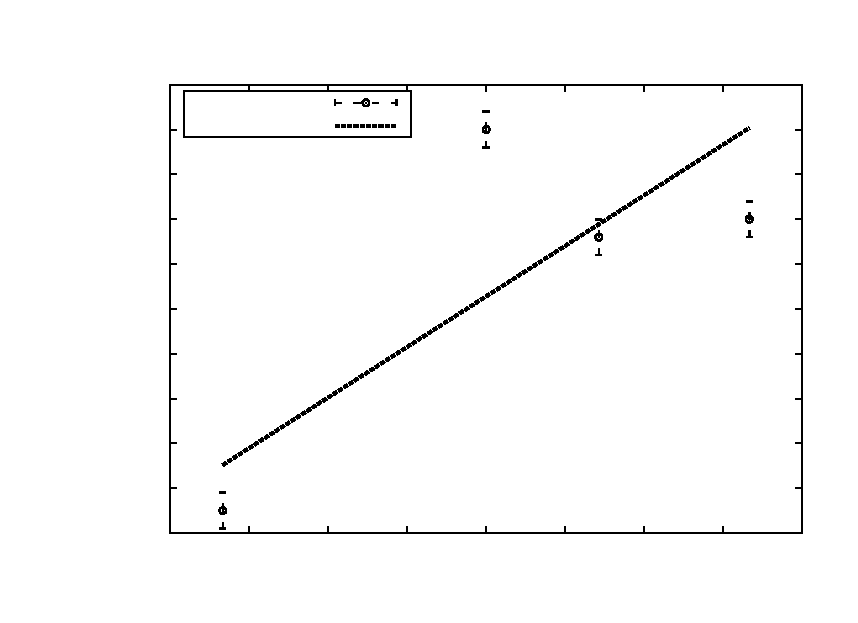
\includegraphics{graph-fenda-dupla}}%
    \gplfronttext
  \end{picture}%
\endgroup

        \caption{gráfico e regressão dos dados de fenda dupla}
        \label{graph-1}  
    \end{subfigure}
   
    \caption{Gráficos}
    
\end{figure}


\FloatBarrier


\subsection{Caracterização de fendas múltiplas}
\paragraph{}Notamos como esperado que o aumento da densidade
de fendas aumenta a distância entre as franjas ao mesmo
tempo em que torna a intensidade destas mais homogêneas.


\paragraph{}

\subsection{Redes de difração}
\paragraph{}Para a rede de valor nominal 600 linhas/mm vamos determinar
a densidade de linhas experimentalmente. Para isso lembremos da fórmula 
\ref{eq:rede} da introdução. Isolando d obtemos:

\begin{equation}
	d = \frac{m \lambda}{sin \theta}
\end{equation}

\paragraph{}Aqui não podemos fazer a aproximação dos ângulos pequenos
que fizemos anteriormente. Fazemos agora
 $\sin \theta =\frac{y_m}{\sqrt{L^2 +y_m^2 }}$
\paragraph{}
Para m = 1 nos dados da tabela \ref{tab:rede}, L =$ (9.00 \pm 0.05)$cm, $y_1 = (35.0 \pm0.5)$mm e $\lambda = 632.8$nm obtemos:

\begin{equation}
\MyBox{	$d = (1.74 \pm 0.04)\mu m$}
\end{equation}

Onde o erro foi obtido pela fórmula:
 
\begin{equation}
	|\triangle(d)| =|(m \lambda) 
		\left[
		  \left(
			\frac{-\sqrt{L^2 + y_m^2}}{y_m^2} + \frac{1}{\sqrt{L^2 + y_m^2}}	 
		  \right)\triangle y_m			
	-	\left(
			\frac{L}{y_m\sqrt{L^2 + y_m^2}}
		\right) \triangle L
		\right] |
\end{equation}

Invertendo d podemos achar N, o número de ranhuras por milímetro:

\begin{equation}
\MyBox{	$N = (575 \pm 10)\mbox{ranhuras por mm}$}
\end{equation}
Onde o erro foi achado por:

\begin{equation}
	|\triangle N| = |\frac{\triangle d}{d^2}|
\end{equation}

\paragraph{} O valor e a margem de erros calculados não incluem o valor nominal
informado pelo fabricante. A margem de erro é de cerca de 1.7\% da melhor
medida. O procedimento foi portanto preciso mas não acurado.

\subsection{Determinação de espectros}
\paragraph{}Usamos agora o valor de d calculado no procedimento anterior
para achar os lambdas que compõe a luz examinada na fonte de mercúrio. A fórmula
para o cálculo é $\lambda = \frac{d \sin \theta}{m}$. A tabela a seguir
resume os resultados, nas primeiras cinco linhas temos m = 1, e nas últimas
m = 2.
\FloatBarrier
\begin{table}[!htp]
\centering
\begin{tabular}{|l|l|}\hline
	$\theta \pm 0.1º$  & $\lambda$  \\ \hline
         14.0º	 &$( 421 \pm 10 )$nm \\ \hline
	 15.1º & $( 453 \pm 10 )$nm \\ \hline
	 17.1º & $( 512 \pm 10 )$nm \\ \hline
 	 19.1º & $( 569 \pm 20 )$nm \\ \hline
	 20.1º & $( 598 \pm 20 )$nm \\ \hline
	 29.2º & $( 424 \pm 10 )$nm \\ \hline
	 31.5º & $( 453 \pm 10 )$nm \\ \hline
	 36.3º & $( 515 \pm 10 )$nm \\ \hline
	 41.0º & $( 571 \pm 10 )$nm \\ \hline
	 43.9º & $( 603 \pm 10 )$nm \\ \hline
\end{tabular}
\end{table}
\FloatBarrier
Onde o erro foi calculado usando a fórmula:
\begin{equation}
	\triangle \lambda =
 \frac{\sin \theta}{m} \triangle d + \frac{d}{m} \cos \theta \triangle \theta
\end{equation}
*tomou-se o devido cuidado de na fórmula acima usar a variação de$\theta$ em 
radianos e não em graus.

\paragraph{}Vemos que todos os valores para m=1 coincidem com os valores
para m=2. Além disso as margens de erro todas abaixo de 4\%. As medidas são
então precisas. Segundo a referência [5] o espectro do mercúrio contém os 
seguintes comprimentos de onda(tradução livre):

 "435.835 nm (azul), 546.074 nm (verde), e um par
em 576.959 nm e 579.065 nm (amarelo-laranja). Existe duas outras linhas azuis em
 404.656 nm e 407.781 nm e uma linha fraca  491.604 nm. "

\paragraph{}Comparando os valores vemos que tanto os valores de m=1 como m=2
acertam os comprimentos de 576 e 579 tabelados mas falham nos outros. O 
procedimento não é portanto acurado.

\subsection{Dispersão em um prisma}
\paragraph{}Nota-se  em
comparação com a dispersão em rede de difração que no caso do prisma a fenda
volta a aparecer somente em uma direção angular(no caso, a
horária). Na dispersão devido a rede achávamos a fenda ao
girar o telescópio nas duas direções. Outra diferença está
na ordem em que as cores aparecem. No caso da dispersão a
primeira cor a aparecer ao nos distanciarmos do 0 angular
era o azul e a última o laranja, no caso do prisma é
justamente o contrário. Outra observação é que o prisma
separa muito menos as cores, cores próximas aparecem como um
só, sendo possível destingir apenas 
3 faixas, enquanto a rede permite 5.

\paragraph{}A diferença no comportamento da sequência de
cores se deve a natureza do processo que as separas. No caso
da rede a separação ocorre devido a difração e a
interferência enquanto no prisma a separação ocorre devido a
refrações do feixe na entrada e na saída do material.

\subsection{Discutindo o erro}
\paragraph{}Vemos que tanto o procedimento para se medir
a densidade de fendas como para medir o espectro de emissão
do mercúrio geram margens de erro baixas e portanto o
procedimento é preciso. Os valores achados estão todos na 
mesma ordem de grandeza que os tabelados mas as margens de
erro encontradas não incluem estes, o experimento portanto
não foi acurado. 

\paragraph{}Uma fonte de erro que deve ter gerado essa
discrepância dos resultados com os valores esperados é o
método de aquisição dos dados. Mais especificamente, a
marcação das franjas no papel milimetrado foi feita
manualmente e de forma a gerar grandes imprecisões. O papel
milimetrado se encontrava fixo ao anteparo por fita adesiva
mas o próprio anteparo não estava muito fixo à base, podendo
girar em torno de seu eixo. Ao se apoiar sobre a mesa para
desenhar a área brilhante sobre o papel diversas vezes
não se pôde evitar
de que a posição do anteparo fosse modificada ao longo do
procedimento. Temos portanto que os dados do papel
milimetrado não são tão precisos quanto a divisão desse nos 
leva a crer. Além claro da dificuldade de se traçar linhas
em uma pepel apoiado verticalmente.

\paragraph{}Outra fonte de erro são as imperfeições nos
slides, mais criticamente no slide de fendas duplas. O laser
difratado
que deveria formar pontos isolados sobre a tela acabava por
'pintar' grande parte da tela, sendo difícil identificar
algumas vezes o que era ruído e o que era padrão de
difração.

\paragraph{}Pode-se concluir da margem de erro achada e da
discrepância encontrada que procedimentos que usam o efeito
da difração e da interferência podem ser usados para obter
medidas muito precisas, da ordem de frações de micrômetros,
mas que deve-se ter muito cuidado com o procedimento pois 
pequenos erros na amostragem dos dados irão gerar resultados
errôneos.
%@@@@@@@@@@@@@@@@@@@@@@@@@@@@@@@@@@@@@@@@@@@@@@@@@@@@@@@@@@@
%@@@@@@@@@@@@@@       CONCLUSÃO       @@@@@@@@@@@@@@@@@@@@@@
%@@@@@@@@@@@@@@@@@@@@@@@@@@@@@@@@@@@@@@@@@@@@@@@@@@@@@@@@@@@
\section{Conclusão}

\paragraph{}O experimento permitiu estudar e caracterizar 
os diferentes padrões de interferência e difração de luz e
reforça o caráter ondulatório da luz. Concluiu-se que em
fenda simples a largura do máximo central aumenta com a 
diminuição da abertura da fenda, em fenda dupla o aumento
da separação das fendas faz as franjas se aproximarem e
em fendas múltiplas o aumento da densidade de fendas
distancia as franjas. Foi possível medir a densidade
de fendas de um slide em N =$575 \pm 10\frac{fendas}{mm}$ e esse dado foi
usado para se obter o espectro de uma lâmpada
de mercúrio. O espectro obtido contém a os comprimentos de
onda 421nm, 453nm,512nm,596nm,598nm todos com margem de erro  
em torno de 4\%. As margens de erro obtidas mostram que o 
procedimento é preciso mas os valores achados divergiram
todos dos valores tabelados, o experimento falhou
portanto em acurácia. Por fim, foi possível verificar
a diferença entre a dispersão causada por difração em rede
de fendas e a causada por refração em prisma, observando-se
que a primeira é muito mais eficiente para se dividir um
espectro do que a segunda.
%@@@@@@@@@@@@@@@@@@@@@@@@@@@@@@@@@@@@@@@@@@@@@@@@@@@@@@@@@@@
%@@@@@@@@@@@@@@       REFERÊNCIAS     @@@@@@@@@@@@@@@@@@@@@@
%@@@@@@@@@@@@@@@@@@@@@@@@@@@@@@@@@@@@@@@@@@@@@@@@@@@@@@@@@@@
\begin{thebibliography}{9}    
	 \bibitem{fis4-serway}
  		JEWETT, J.W.; SERWAY, R.A.
  		\emph{Física para cientistas e engenheiros}
volume 4 : Luz, Óptica e Física Moderna.
 		 8ª ed.
 		 São Paulo : Cengage Learning, 2012.
 		 
	\bibitem{wiki: Huygens}
 		Autor desconhecido. Huygens–Fresnel principle. Disponível
em: http://en.wikipedia.org/wiki/Huygens$\%E2\%80\%93Fresnel\_principle$.
Acesso em: 3 de Julho de 2013
  	
  	\bibitem{figura usada}Bill Casselman at UBC:
The University of British Columbia. 
  	SINGLE SLIT DIFFRACTION PATTERN OF LIGHT	 
  	Disponível em:
	http://www.math.ubc.ca/~cass/courses/m309-03a/m309-projects/krzak/.
  	Acesso em 4 de Julho de 2013.
  		
  	\bibitem{MIT: cap14}
  	MIT, notas de aula. Electromagnetism, chapter 14:
			 Interference and Diffraction. Disponível em: 
       http://web.mit.edu/viz/EM/visualizations/coursenotes/modules/guide14.pdf.
	 Acesso em 4 de Julho de 2013.

	\bibitem{Hg}
	R, Nave. Hyperphysics,Atomic Spectra. 
	Disponível em :
http://hyperphysics.phy-astr.gsu.edu/hbase/quantum/atspect2.html\#c2
	Acesso em 12 de Julho de 2013.
  		
\end{thebibliography}
\end{document}
